\documentclass[ 
	12pt,
	a4paper,
	bibtotoc,
	cleardoubleempty, 
	idxtotoc,
	ngerman, 
	openright
	final, 
	listof=nochaptergap,
	]{scrbook}

\usepackage[T1]{fontenc}
\usepackage[utf8]{inputenc}
  
% ##################################################
% Unterstuetzung fuer die deutsche Sprache
% ##################################################
%\usepackage{ngerman}
\usepackage[ngerman]{babel}

% ##################################################
% Dokumentvariablen
% ##################################################

% Persoenliche Daten
\newcommand{\docB}{Ann-Sophie Dietrich}
\newcommand{\docA}{Jan-Henrik Preuß}
\newcommand{\docC}{Marcel Schlipf}
\newcommand{\docD}{Christian Würthner}

% Dokumentdaten
\newcommand{\docTitle}{Webserver für ein embedded Board mit AVR-Prozessor}
%\newcommand{\docUntertitle}{} % Kein Untertitel
\newcommand{\docUntertitle}{Dokumentation}
% Arten der Arbeit: Bachelorthesis, Masterthesis, Seminararbeit, Diplomarbeit
\newcommand{\docArtDerArbeit}{Projektarbeit}
%Studiengaenge: Allgemeine Informatik Bachelor, Computer Networking Bachelor,
% Software-Produktmanagement Bachelor, Advanced Computer Scinece Master
\newcommand{\docStudiengang}{AIB/CNB}
\newcommand{\docAbgabedatum}{30.07.2014}
\newcommand{\docErsterReferent}{Dr. Jiri Spale}
%\newcommand{\docZweiterReferent}{-} % Wenn es nur einen Betreuer gibt
%\newcommand{\docZweiterReferent}{ZWEITER REFERENT}

% ##################################################
% Allgemeine Pakete
% ##################################################

% Abbildungen einbinden
\usepackage{graphicx}

% Zusaetsliche Sonderzeichen
% \usepackage{dingbat}

% Farben
\usepackage{color}
\usepackage[usenames,dvipsnames,svgnames,table]{xcolor}

% Maskierung von URLs und Dateipfaden
\usepackage[hyphens]{url}

% Deutsche Anfuehrungszeichen
\usepackage[babel, german=quotes]{csquotes}

% Pakte zur Index-Erstellung (Schlagwortverzeichnis)
\usepackage{index}
\makeindex

% Ipsum Lorem
% Paket wird nur für das Beispiel gebraucht und kann gelöscht werden
\usepackage{lipsum}

% ##################################################
% Seitenformatierung
% ##################################################
\usepackage[
	portrait,
	bindingoffset=1.5cm,
	inner=2.5cm,
	outer=2.5cm,
	top=3cm,
	bottom=2cm,
	%includeheadfoot
	]{geometry}

% ##################################################
% Kopf- und Fusszeile
% ##################################################

\usepackage{fancyhdr}

\pagestyle{fancy}
\fancyhf{}
\fancyhead[EL,OR]{\sffamily\thepage}
\fancyhead[ER,OL]{\sffamily\leftmark}

\fancypagestyle{headings}{}

\fancypagestyle{plain}{}

\fancypagestyle{empty}{
  \fancyhf{}
  \renewcommand{\headrulewidth}{0pt}
}

%Kein "Kapitel # NAME" in der Kopfzeile
\renewcommand{\chaptermark}[1]{
	\markboth{#1}{}
   	\markboth{\thechapter.\ #1}{}
}

% ##################################################
% Schriften
% ##################################################

% Stdandardschrift festlegen
\renewcommand{\familydefault}{\sfdefault}

% Standard Zeilenabstand: 1,5 zeilig
\usepackage{setspace}
\onehalfspacing 

% Schriftgroessen festlegen
\addtokomafont{chapter}{\sffamily\large\bfseries} 
\addtokomafont{section}{\sffamily\normalsize\bfseries} 
\addtokomafont{subsection}{\sffamily\normalsize\mdseries} 
\addtokomafont{caption}{\sffamily\normalsize\mdseries} 

% ##################################################
% Inhaltsverzeichnis / Allgemeine Verzeichniseinstellungen
% ##################################################

\usepackage{tocloft}

% Punkte auch bei Kapiteln
\renewcommand{\cftchapdotsep}{3}
\renewcommand{\cftdotsep}{3}

% Schriftart und -groesse im Inhaltsverzeichnis anpassen
\renewcommand{\cftchapfont}{\sffamily\normalsize}
\renewcommand{\cftsecfont}{\sffamily\normalsize}
\renewcommand{\cftsubsecfont}{\sffamily\normalsize}
\renewcommand{\cftchappagefont}{\sffamily\normalsize}
\renewcommand{\cftsecpagefont}{\sffamily\normalsize}
\renewcommand{\cftsubsecpagefont}{\sffamily\normalsize}

%Zeilenabstand in den Verzeichnissen einstellen
\setlength{\cftparskip}{.5\baselineskip}
\setlength{\cftbeforechapskip}{.1\baselineskip}

% ##################################################
% Abbildungsverzeichnis und Abbildungen
% ##################################################

\usepackage{caption}

\usepackage{wrapfig}

% Nummerierung von Abbildungen
\renewcommand{\thefigure}{\arabic{figure}}
\usepackage{chngcntr}
\counterwithout{figure}{chapter}

% Abbildungsverzeichnis anpassen
\renewcommand{\cftfigpresnum}{Abbildung }
\renewcommand{\cftfigaftersnum}{:}

% Breite des Nummerierungsbereiches [Abbildung 1:]
\newlength{\figureLength}
\settowidth{\figureLength}{\bfseries\cftfigpresnum\cftfigaftersnum}
\setlength{\cftfignumwidth}{\figureLength}
\setlength{\cftfigindent}{0cm}

% Schriftart anpassen
\renewcommand\cftfigfont{\sffamily}
\renewcommand\cftfigpagefont{\sffamily}

% ##################################################
% Tabellenverzeichnis und Tabellen
% ##################################################

% Nummerierung von Tabellen
\renewcommand{\thetable}{\arabic{table}}
\counterwithout{table}{chapter}

% Tabellenverzeichnis anpassen
\renewcommand{\cfttabpresnum}{Tabelle }
\renewcommand{\cfttabaftersnum}{:}

% Breite des Nummerierungsbereiches [Abbildung 1:]
\newlength{\tableLength}
\settowidth{\tableLength}{\bfseries\cfttabpresnum\cfttabaftersnum}
\setlength{\cfttabnumwidth}{\tableLength}
\setlength{\cfttabindent}{0cm}

%Schriftart anpassen
\renewcommand\cfttabfont{\sffamily}
\renewcommand\cfttabpagefont{\sffamily}

% Unterdrueckung von vertikalen Linien
\usepackage{booktabs}

%Fluss eigenschaften von Tabellen

\usepackage{float}

% ##################################################
% Listings (Quellcode)
% ##################################################

\usepackage{listings}
\lstset{
	language=java,
	backgroundcolor=\color{white},
	breaklines=true,
	prebreak={\carriagereturn},
 	breakautoindent=true,
 	numbers=left,
 	numberstyle=\tiny,
 	stepnumber=2,
 	numbersep=5pt,
 	keywordstyle=\color{blue},
   	commentstyle=\color{green},   
   	stringstyle=\color{gray}
}
  	
% ##################################################
% Theoreme
% ##################################################
  	
% Umgebung fuer Beispiele
\newtheorem{beispiel}{Beispiel}

% Umgebung fuer These
\newtheorem{these}{These}

% Umgebung fuer Definitionen
\newtheorem{definition}{Definition}
  	
% ##################################################
% Literaturverzeichnis
% ##################################################

\usepackage{bibgerm}

% ##################################################
% Abkuerzungsverzeichnis
% ##################################################

\usepackage[printonlyused]{acronym}

% ##################################################
% PDF / Dokumenteninternelinks
% ##################################################

\usepackage[
	colorlinks=false,
   	linkcolor=black,
   	citecolor=black,
  	filecolor=black,
	urlcolor=black,
    bookmarks=true,
    bookmarksopen=true,
    bookmarksopenlevel=3,
    bookmarksnumbered,
    plainpages=false,
    pdfpagelabels=true,
    hyperfootnotes,
    pdftitle ={\docTitle},
    pdfauthor={\docVorname~\docNachname},
    pdfcreator={\docVorname~\docNachname}]{hyperref}
 
\begin{document}

\setcounter{secnumdepth}{3}
 
% Titelblatt
\begin{titlepage}
\pagestyle{empty}

% ##################################################
% HFU-Logo einbinden
% ##################################################
\begin{flushright}
\begin{figure}[ht]
\flushright

\includegraphics[height=3cm]{content/pictures/hfu.jpg}
\end{figure}
\end{flushright}

% ##################################################
% Titel
% ##################################################
\begin{center}
{\fontsize{18}{22} \selectfont \docArtDerArbeit}\\[5mm]
{\fontsize{18}{22} \selectfont im Studiengang} \\[5mm]
{\fontsize{18}{22} \selectfont \docStudiengang}\\
\vspace{1cm}
\begin{onehalfspace}
{\fontsize{22}{26} \selectfont \textbf{\docTitle}}\\[5mm]
{\fontsize{18}{22} \selectfont \docUntertitle}


\end{onehalfspace}
\end{center}

% ##################################################
% Zusatzinformationen
% ##################################################
\vfill
\begin{center}
\begin{tabular}{lcl}
Referent  		&:& \docErsterReferent 	\\ \\
Vorgelegt am 	&:& \docAbgabedatum 	\\ \\
Vorgelegt von 	&:& \docA\\
				&&	\docB\\
				&&	\docC\\
				&&	\docD\\		
\end{tabular}
\end{center}
\end{titlepage}
\cleardoubleemptypage

\frontmatter



% Abstract
\chapter*{Abstract\markboth{Abstract}{}}
\addcontentsline{toc}{chapter}{Abstract}
Die Aufgabe des Semesterprojektes bestand darin, auf einem Pollin-Net-IO-Board, auf welchem als Prozessor ein ATmega644p 
läuft, einen Webserver aufzusetzen. Als Vorlage für den Webserver gab es eine Version von Ulrich Radig, welche man nutzen, verbessern und ausbauen soll.\\
Mit Hilfe des Webservers soll es möglich sein, den Status der sich auf dem Board 
befindenden Pins anzeigen und diese manipulieren zu lassen. Die Anzeige, sowie die Manipulation soll über eine Webseite, 
auf welcher das Board grafisch dargestellt wird geschehen. Zudem soll man pro Pin auf der Webseite eine Beschreibung und Funktion 
hinterlegen, welche gespeichert bleibt und abrufbar ist. Die Webseite soll den aktuellen Platinenstand grafisch anzeigen, änderungen am Board sollen so 
schnell es möglich ist auf der Webseite grafisch angezeigt werden.\\

\cleardoubleemptypage

% Inhaltsverzeichnis
\tableofcontents
\addcontentsline{toc}{chapter}{Inhaltsverzeichnis}
\cleardoubleemptypage

% Abbildungsverzeichnis einbinden und ins Inhaltsverzeichnis
% WORKAROUND: tocloft und KOMA funktionieren zusammen nicht
% korrekt\phantomsection
\addcontentsline{toc}{chapter}{\listfigurename} 
\listoffigures
\cleardoubleemptypage

% Tabellenverzeichnis einbinden und ins Inhaltsverzeichnis
% WORKAROUND: tocloft und KOMA funktionieren zusammen nicht
% korrekt\phantomsection
\phantomsection
\addcontentsline{toc}{chapter}{\listtablename}
\listoftables
\cleardoubleemptypage

% Abkürzungsverzeichnis
\chapter*{Abkürzungsverzeichnis\markboth{Abkürzungsverzeichnis}{}}
\addcontentsline{toc}{chapter}{Abkürzungsverzeichnis}

\begin{acronym}
\acro{AJAX}{Asynchronous JavaScript and XML}
\acro{DDR}{Data Direction Register}
\acro{EEPROM}{Electrically Erasable Programmable Read-Only Memory}
\acro{HFU}{Hochschule Furtwangen University}
\acro{HHC}{HTML Header Compiler}
\acro{HTML}{Hyper Text Markup Language}
\acro{HTTP}{Hyper Text Transfer Protocol}
\acro{IDE}{Integrated Development Environment}
\acro{ISP}{In System Programming}
\acro{JSON}{JavaScript Object Notation}
\acro{JTAG}{Joint Test Action Group}
\acro{REST}{Representational State Transfer}
\acro{RSS}{Rich Site Summary}
\acro{SOAP}{Simple Object Access Protocol}
\acro{SPI}{Serial Peripheral Interface}
\acro{URL}{Uniform Resource Locator}
\acro{WDT}{Watchdog timer}
\acro{XML}{Extensible Markup Language}
\end{acronym}


\mainmatter

\chapter{Einleitung}

Durch die weiter fortschreitende Vernetzung unserer alltäglichen Elektronik
wird das verlangen nach netzwerkfähigen Mikrocontrollern
immer wichtiger. Wenn der moderne Kühlschrank erkennen soll, wie gut er gerade
gefüllt ist oder wenn die Heizung melden soll wie warm das Wasser ist, muss ein
entsprechend ausgestatteter Controller diese Informationen an den Nutzer
melden können. Hier greift unser Projekt da mit dem Mikrocontroller und seinen
verschiedenen ein und Ausgängen unterschiedlichste Anwendungen ermöglicht
werden. 

\chapter{Grundlagen}
%http://samurai1967.dyndns.org/avr-net-io.html
%http://www.fhemwiki.de/wiki/AVR-NET-IO
%http://www.mikrocontroller.net/articles/AVR_Net-IO_Bausatz_von_Pollin
\section{AVR Net-IO-Board}
\begin{figure}[h]
\centering
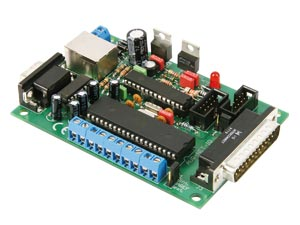
\includegraphics[width=10cm]{content/pictures/avr-net-io.jpg}
\caption{AVR-NET-IO - Pollin GmbH}
%http://www.pollin.de/shop/dt/MTQ5OTgxOTk-/Bausaetze_Module/Bausaetze/Bausatz_AVR_NET_IO.html
\label{fig:B3}
\end{figure}

\subsection{Technische Daten}
\begin{itemize}
  \item Betriebsspanne 9V
  \item Stromaufnahme ca. 190 mA
  \item 8 Digitale Ausgänge, 4 Digitale Eingänge
  \item 4 Analoge Eingänge
  \item ATmega32 Mikrocontroller
  \item integrierte ISP-Schnittstelle
\end{itemize}

\section{Mikrocontroller}
\subsection{ATmega32}

\subsection{ATmega644P}

\subsection{ATmega1284P}


\chapter{System Architektur}

\begin{itemize}
\item Was soll hier rein??
\end{itemize}
\chapter{Tutorial} %Soll der name verwendet werden? [janp]

\section{Einrichten eines neuen Microcotrollers}
Für unser Projekt sollen alle notwendigen Programmbestandteile sowie die gesamte
Website auf dem Microcotnroller gespeichert werden. Der beim AVR-Net-IO
mitgelieferte ATmega32 bietet hierfür jedoch nicht ausreichend Speicher.
Wir haben uns deswegen für den aus der gleichen Baureihe stammenden ATmega644P
entschieden der mit seinen 64KB Programmspeicher den doppelten Speicherplatz
bietet als der kleinere ATmeag32.

Für einen neuen Chip ist es anfangs notwendig die Fuse-Bits richtig zu setzen,
damit der Chip Ordnungsgemäß Arbeitet.
Dies ist jedoch im AtmelStudio nicht Möglich, da es nicht möglich ist die exakte
Geräte-Signatur auszulesen.
Das Problem liegt darin, das Standartmäßig die Fuses auf den internen
Quarz-Kristall gesetzt sind und nicht auf den Externen Kristall des
AVR-NET-IO Boards.
Beim versuch die Fuse-Bits zu setzen wird man im Atmel Studio mit folgender
Fehlermeldung begrüßt. 
\begin{figure}[h]
\centering
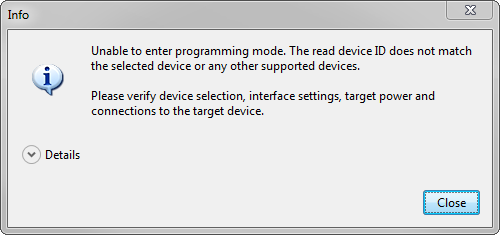
\includegraphics[width=13cm]{content/pictures/Anleitung/neuerProzessor/AnleitungNeuerProzessor2_fehler.png}
\caption{DeviceProgramming}
\end{figure}

Abhilfe Schafft hier die Alternative Programmiersoftware AVRDUDE, mit ihr ist
es Möglich die Fuse-Bits zu ändern. Unter Linux kann dieser einfach über die
Paketquellen installiert werden, für ein Windows Betriebssystem kann eine
ausführbare Kommandozeilen-Anwendung auf der Projekt-Website heruntergeladen
werden \url{http://savannah.nongnu.org/projects/avrdude}. 

\begin{table}[H]
\begin{tabular}{| p{.24\textwidth} | p{.76\textwidth} |}
\hline
Auslesen Linux:& sudo avrdude -P usb -p m644p -c avrispmkII  -U lfuse:r:-:h -U hfuse:r:-:h -B 22 \\ \hline
Setzen Linux:& sudo avrdude -P usb -p m644p -c avrispmkII -U lfuse:w:0xFF:m -U hfuse:w:0xD6:m -B 22 \\ \hline
% Auslesen Windows:& avrdude.exe -p m644p -c avrispmkII -U lfuse:r:-:h -U hfuse:r:-:h -B 22 \\ \hline 
% Setzen Windows:& avrdude.exe -p m644p -c avrispmkII -U lfuse:w:0xFF:m -U hfuse:w:0xD6:m -B 22 \\ \hline
%
% Muss noch getestet werden!
%
\end{tabular}
\caption{Auslesen und setzen von Fuse-Bits mit dem AVRDUDE}
\label{tablelabel}
\end{table}

Ein Auszug der verwendeten Parameter aus der AVRDUDE Handbuch Seite.

\begin{table}[H]
\begin{tabular}{| p{.35\textwidth} | p{.65\textwidth} |}
\hline
-p partno & This is the only option that is mandatory for every invocation of
avrdude.  It specifies the type of the MCU connected to the programmer. These
are read from the config file.  If avrdude does not know about a part that you
have, simply add it to the config file (be sure and submit a patch back to the
author so that it can be incorporated for the next version). \newline
\textbf{m32 $\Rightarrow$ ATmega32} \newline 
\textbf{m644p $\Rightarrow$ ATmega644P} \newline
\textbf{m1284p $\Rightarrow$ ATmega1284P} \\ \hline
-P port & Use port to identify the device to which the programmer is attached. \textbf{usb für den AVRISP MKII}  \\ \hline 
-c programmer-id & \textbf{avrispmkII für den AVRISP MKII} \\ \hline
-U \hbox{memtype:op:filename:filefmt} &  
The \textrm{memtype} field specifies the memory type to operate on.\newline
\textbf{hfuse} The high fuse byte.\newline
\textbf{lfuse} The low fuse byte.\newline
The \textrm{op} field specifies what operation to perform:\newline
\textbf{r} read device memory and write to the specified file\newline
\textbf{w} read data from the specified file and write to the device memory \newline
The filename field indicates the name of the file to read or write.  The format field is optional and contains the format of the file to read or write. \newline
\textbf{Hier die Bytes die gesetzt werden 0xFF bzw 0xD6}
\\ \hline
-B bitclock & Specify the bit clock period for the JTAG interface or the ISP clock \\ \hline
\end{tabular}
\caption{Auslesen und setzen von Fuse-Bits mit dem AVRDUDE}
\label{tablelabel}
\end{table}

Die Ausgabe von AVRDUDE beim setzen der neuen Fuse-Bit Einstellungen.

\begin{figure}[h]
\centering
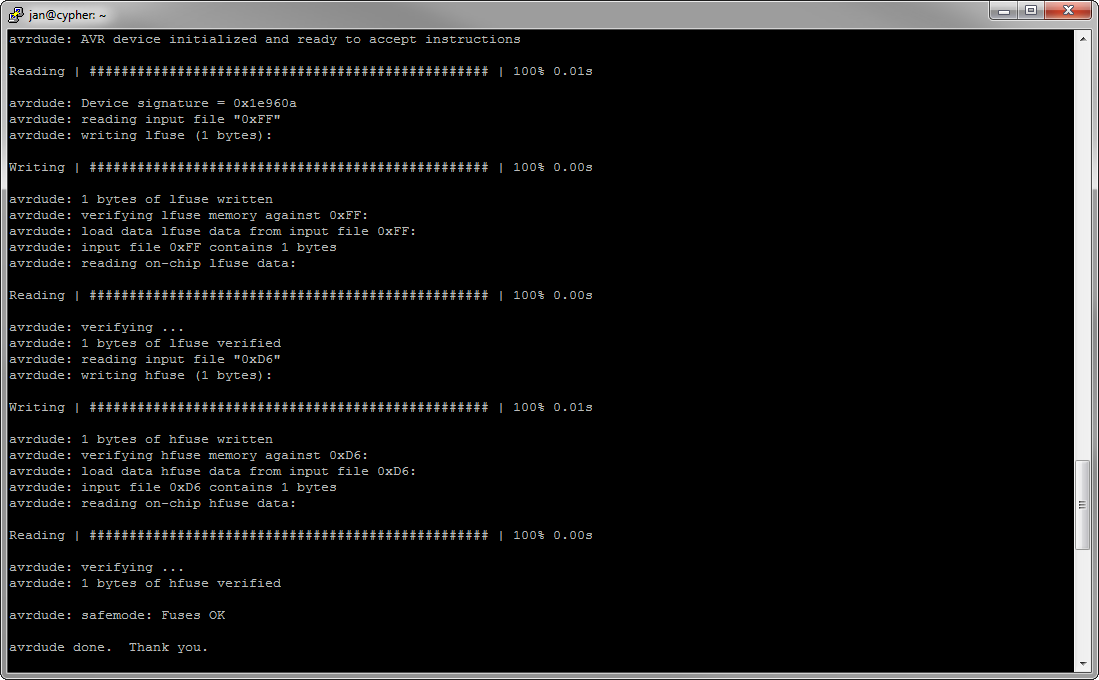
\includegraphics[width=13cm]{content/pictures/Anleitung/neuerProzessor/avrOutput.png}
\caption{AVRDUDE Ausgabe}
\end{figure}

Anschließend kann der Mikrocontroller zusammen mit dem AV-Net-IO und AtmelStudio Programmiert werden. 



\section{Konfiguration}

Einstellen von:
IP
Mac
Ein/Ausgänge


\section{HTML Header Compiler}

Parameter und Funktionsweise

\section{Hexfiles Überspielen}

Zum übertragen der Hexfiles gibt es verschiedene Möglichkeiten.

\subsection{AVRDUDE}



\subsection{Atmel Studio}

\section{Die Website}

\chapter{Werkzeuge}

\section{Das Atmel Studio}

\subsection{DeviceProgramming}

Gerät Auswählen
Contoller Auswählen
Spannung und Signatur
Fuse Bits
Hexfile Flashen

\begin{figure}[h]
\centering
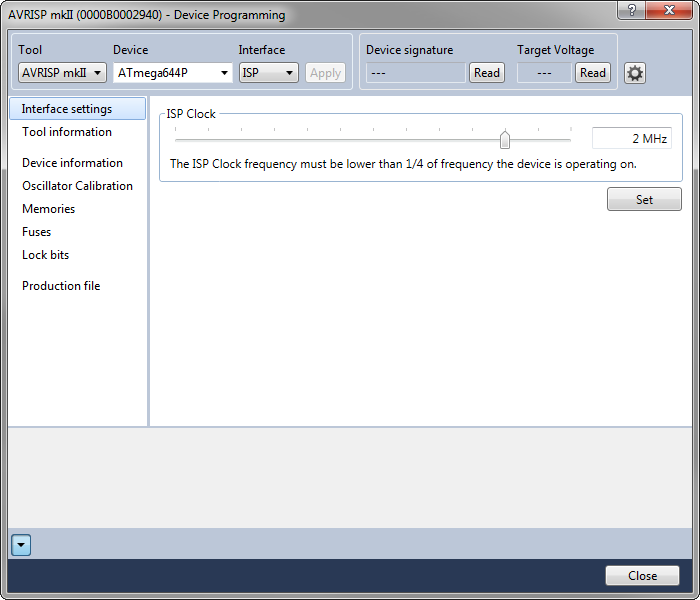
\includegraphics[width=13cm]{content/pictures/Anleitung/neuerProzessor/AnleitungNeuerProzessor1.png}
\caption{DeviceProgramming}
\label{fig:B3}
\end{figure}

\section{Projekt Einstellungen}

Taktfrequenz
Programmer
Empfolene Tool Settings

\section{AVRDUDE}

\section{HTML Header Compiler}
\chapter{Der Webserver}

Als Basis für unser Projekt haben wir die Firmware von Ulrich Radig verwendet.
Da diese Vorlage für unseren Anwendungsfall zu umfangreich ist,  haben wir uns 
für die Abgespeckte Variante von Günther Menke entschieden. Die Änderungen sind
zum einen das entfernte Kamera-Feature und um zusätzlichen Quellcode für einen
alternativen Netzwerkcontroller abgespeckt wurde.

\section{Einrichtung}

Die Einstellung des Webservers erfolgt über die \textrm{config.h} Datei. Hier können
IP-Adresse, Mac-Adresse oder die Ports eingestellt werden.

\section{Einbindung der Website}

Alle für den Betrieb der Website benötigten Dateien sind nicht über ein
Dateisystem vorhanden, sondern werden beim zugriff des Benutzers auf den
Webserver über die \textrm{webpage.h} datei geladen.
Das erstellen der .h erfolgt über das Beigelegte \textrm{HTML Header Compiler}
Werkzeug erstellt. Eine Beispiel zum erstellen der \textrm{webpage.h} Datei gibt
es im Tutorial Abschnitt. Das Werkzeug wird im Kapitel Werkzeuge detailierter
erklärt. Abschließend ist noch zu erwähnen, das die \textrm{webpage.h} nicht für manuelle
Bearbeitung gedacht ist. Dies geschieht ausschließlich über die Quell-Dateien
und dem anschließenden umwandeln mit dem \textrm{HTML Header Compiler}



\include{content/Website}
\chapter{Kommunikation zwischen Server und Webseite}

\section*{Kommunikation im Projekt Radig}
Im Projekt Radig ist keine echte Kommunikation zwischen dem Client und dem Server 
vorhanden. 

Die auf der Webseite dargestellten Werte werden vor dem senden der HTML-Seite 
im HTML-Code eingefügt indem Platzhalter im Format "\%PORTA0" ersetzt und so statisch auf 
der Webseite dargestellt werden. Das Manipulieren der Pins findet über ein HTML-Formular 
statt. Alle manipulierbaren Pins sind als Input vom Typ Checkbox dargestellt. Diese lassen 
sich frei manipulieren und erst beim Betätigen des "Senden"-Buttons werden die 
Informationen per POST-Event an den Server gesendet und so die Seite neu aufgerufen. Der 
Server filtert die POST Informationen aus dem HTTP-Header und manipuliert die Pins gemäß 
den Anweisungen. Beim senden des angeforderten HTML-Dokumentes werden die neuen Werte in 
den HTML-Code eingefügt, und so die neuen Werte auf der Webseite angezeigt.

Das große Problem bei dieser technisch einfachen Lösung ist, das geänderte Werte erst beim 
nächsten neu laden der Webseite angezeigt werden. Ändert sich ein Pin während die Webseite 
dargestellt wird bekommt der Nutzer dies nicht mit. Zudem wird bei jedem Manipulieren 
eines Pins die gesamte Seite neu geladen und so Unmengen an unnötigen Daten übertragen. 
Auch zum darstellen der aktuellen Werte muss die ganze Seite neu vom Server angefordert 
werden.

\section*{Erster Ansatz}
Die Kommunikation zwischen Server und Client sollte mit Hilfe einer REST-Schnittstelle 
stattfinden, die im Hintergrund über Javascript angesprochen werden kann. 

Eine REST-Schnittstelle besteht aus einer oder mehreren virtuellen URLs. Beim Aufruf einer 
solchen URL liefert der Server kein Dokument das gespeichert ist, sondern erzeugt 
dynamisch eine Antwort mit den benötigten Informationen und sendet diese als Antwort 
zurück. Der Server kann beim Aufruf einer URL auch eine Aktion ausführen.

Vorteile der REST-Schnittstelle ist die simple Implementierung, sowohl auf dem Client mit 
JavaScript als auch auf dem Server. Die Inhalte werden mit JSON formatiert, welches einen 
technisches Standart darstellt und sich in JavaScript direkt in ein Objekt umwandeln 
lässt. Auf dem Server ist es einfach mit einem Stringformat immer gleiche JSON Strukturen 
zu erstellen und nur aktuelle Werte einzufügen. Die REST-Schnittstelle lässt sich leicht 
um weitere, neue Funktionalitäten erweitern, indem neue virtuelle URLs erstellt werden die 
vom Client ansprechbar sind.

Die Anforderungen an eine Lösung in diesem Projekt waren vor allem eine möglichst kompakte 
Schnittstelle zu schaffen die wenig Bandbreite verbraucht um eine hohe 
Übertragungsgeschwindigkeit zu ermöglichen trotz des schwachen Servers. Ein besonderes 
Augenmerk war auf die Übertragung der Messwerte zu legen, da diese nicht wie andere 
statische Informationen nur einmalig übertragen werden sondern kontinuierlich erneuert 
werden müssen. Die Schnittstelle sollte gut skalierbar sein. Würde später ein Port für
eine andere Aufgabe zu verwendet werden muss dieser Port ohne Aufwand aus der 
REST-Schnittstelle ausgeschlossen werden können, damit er von außen nicht manipulierbar 
ist und so interne Abläufe auf der Platine nicht gestört werden.

Nach den Anforderungen muss die Schnittstelle folgende Aufgaben ermöglichen:
\begin{itemize}
\item Abfragen der aktuellen Werte aller verwendbaren Pins
\item Abfragen der Konfiguration eines Pins (Eingang oder Ausgang)
\item Abfragen von Allgemeinen Informationen des Boards (IP, Standart-IP, Mac-Adresse,
	Serverversion)
\item Manipulieren aller als Ausgänge geschaltener Pins
\item Manipulieren der Konfiguration eines Pins (als Eingang oder Ausgang setzen)
\item Manipulieren von Servereinstellungen (z.B. IP-Adresse);
\end{itemize}

%\begin{itemize}
%	\item Aufbau als REST-Schnittstelle
%	\begin{itemize}
%		\item Simpel implementierbar
%		\item Technischer Standart
%		\item Fertige Mechaniken in JavaScript
%		\item Leicht erweiterbar um neue Funktionalitäten
%	\end{itemize}
%	\item Anforderungen an eine Lösung:
%	\begin{itemize}
%		\item Möglichst kompakt, wenig Bandbreite soll verbraucht werden
%		\item Messwerte müssen besonders effizient übertragen werden
%		\item Skalierbar - Egal ob ein oder 20 Ports verwendet werden
%		\item Neben Abfragen der Messwerte auch manipulieren der IP, des DDR und der 
%			  Ausgänge
%		\item JSON-Encodiert, direkt in JavaScript Objekt überführbar
%	\end{itemize}
%\end{itemize}

%-----------------------------------------------------------------------------------------
\section*{Polling oder Pushing}
Die aktuellen Werte der Pins müssen bei jeder Änderung vom Server zum Client übertragen 
werden, damit diese auf der Webseite immer korrekt dargestellt werden. Hierfür stehen zwei 
verschiedene Konzepte zur Verfügung wie die Übertragung der Daten initialisiert werden.

\subsection*{Polling}
Bei Polling werden vom Client kontinuierlich die Werte erneut angefordert, indem dieser 
die entsprechende virtuell URL des Servers aufruft. Dies führt dazu, dass viele unnötige 
Date übertragen werden, da sich eventuell nicht bei jedem erneuten anfordern der Werte 
diese auch tatsächlich verändert haben und so die gleichen Datensätze oft mehrmals 
angefordert werden.

Im vergleich zu der Radig-Lösung bietet Polling den Vorteil das die Werte kontinuierlich 
nach geladen und so immer korrekt dargestellt werden während die Webseite dargestellt 
wird. Auch das gesendete Datenvolumen wird dahingehend minimiert, das nur die Nutzdaten 
übertragen werden und nicht der gesamte HTML-Code der Webseite. Polling ist technisch sehr 
einfach zu realisieren, da die Abfrage der Daten einfach zyklisch wiederholt werden.

\subsection*{Pushing}
Bei Pushing wird im Gegensatz zu Polling der Daten nicht vom Client initialisiert sondern 
vom Server. Der Server weiß wann sich die Werte geändert haben und kann dem Client bei 
jeder Änderung gezielt die neuen Daten Übermitteln. Das Übertragen der Daten könnte z.B. 
durch einen Interrupt ausgelöst werden.

Im direkten vergleich zu Polling bietet Pushing verschiedene Vorteile. So wird nicht nur 
das Volumen der übertragenen Daten reduziert indem keine unnötigen Abfragen stattfinden,
sondern die neuen Werte gelangen auch genau dann zum Client wenn die Änderung tatsächlich 
stattgefunden hat, was dazu führt das die Webseite schneller auf Änderungen reagiert.

Die technische Umsetzung von Pushing ist mit diversen Problemen verbunden. Die typische 
Verbindungsaufbaurichtung ist bei Webanwendungen und Webseiten immer vom Client zum 
Server. Anders als bei Polling müssen bei Pushing Daten vom Server zum Client gelangen. 
Hierfür muss eine Verbindung vom Server zum Client aufgebaut werden. Dies ist technisch 
aber nicht möglich, da der Browser bzw. JavaScript keine Möglichkeit haben einen Port des 
Clientsystems zu öffnen und auf eingehende Verbindungen des Servers zu antworten. 

Das Problem lässt sich durch die Benutzung von HTML5 Server-Sent Events umgehen. Hierbei 
frägt der Client eine virtuelle URL des Servers ab, ähnlich einer REST-Schnittstelle. Der 
Server überträgt jedoch nicht sofort Daten, sondern schreibt erst bei einem Event (z.B. 
die Änderung eines Pins) in den geöffneten Stream und pusht so die Daten zum Client. 
Dieser überwacht den Stream mit Hilfe von JavaScript un empfängt so die neuen Werte und 
kann sie auf der Webseite anzeigen.

Dieses System ist auf dem Pollin Net-IO Board aber nur schwer umzusetzen da mehrere 
Verbindungen verwaltet werden müssen. So ist immer mindestens eine Server-Sent Event 
Verbindung offen, parallel könnte aber ein Client andere Daten vom Server anfordern. Für 
das Verwalten mehrerer Verbindungen sind aber viele Resourcen nötig, da für jede 
Verbindung auch Daten im RAM hinterlegt werden müssen. Außerdem st in vielen Situationen 
ein simples Multitasking nötig, das so auf einem ATmega CPU nicht vorhanden ist. Das Radig 
Projekt setzt aus diesen Gründen auf HTTP 1.0 bei dem für jede Anfrage eine Verbindung 
geöffnet und nach erfolgreichem Übertragen der Daten wieder geschlossen wird. So ist auch 
die Kommunikation mit mehreren Clients problemlos möglich.

Um HTML5 Server-Sent Events auf dem Pollin Net-IO Board zu implementieren würde es als 
einen tendenziell größeren CPU erfordern mit dem auch Multitasking möglich ist sowohl auch 
eine grundlegende Umgestaltung des Radig-Projektes um mehrere HTTP Verbindungen parallel 
zu ermöglichen.

\subsection*{Entscheidung}
Da die technische Umsetzung vom Pushing nur schwer möglich ist werden wir auf Polling 
setzen.

TODO: Hier noch Argumentation mit Übertragungszeit und Screenshot aus Chrome Network Log


%\begin{itemize}
%	\item Daten können entweder per Polling vom Client (Webseite abgefragt werden) oder
%		  vom Server bei einem Event (Änderung eines Eingangs) per Push geschickt werden	  
%	\item Pro/Contra Push
%	\begin{itemize}
%		\item Pro: Daten werden nur übertragen wenn es wirklich nötig ist, kein unnötiger 
%			  Datenverkehr
%		\item Pro: Leistung bleibt auch mit mehreren Clients eher konstant 
%			  (Genau Begründung ausarbeiten!)
%		\item Pro: Board wird entlastet, kein DOS, mehrere Clients können Webseite 
%		      trotzdem problemlos aufbauen 
%	\end{itemize}
%	\item Pro/Contra Polling
%	\begin{itemize}
%		\item Pro: Leichter zu implementieren - normale Dateiabfrage
%		\item Contra: Es werden viele unnötige Daten übertragen
%		\item Contra: Leistung nimmt mit steigender Anzahl von Clients ab
%		\item Pro: Im Prinzip nicht langsamer als Push: Limitierende Komponente ist die 
%			  Übertragungszeit! (Hier Bild von Chrome Netzwerkvehrkehr) 
%	\end{itemize}
%	
%	\item Push bessere Lösung
%	\item Umsetzung aber nicht möglich
%	\item Server kann keine Verbindung zu Client aufbauen
%	\begin{itemize}
%		\item Javascript kann keinen Serverport öffnen
%		\item Client hat keine öffentliche IP
%	\end{itemize}
%	\item Technische Lösung: HTML 5 Server Sent Events
%	\begin{itemize}
%		\item Technischer Standart, Eingeführt mit HTML 5
%		\item Client ruft virtuelle URL auf, ähnlich REST
%		\item So wird ein Stream geöffnet
%		\item Bei einem Event schreibt der Server die Informationen in den Stream
%		\item Client benutzt Javascript API um die jeweiligen Informationen zu lesen
%	\end{itemize}
%	\item Mit ATmega CPU und Radig Projrkt als Vorlage nicht lösbar
%	\begin{itemize}
%		\item Radig kann nur eine Verbindung handeln. Aufbau - Übertragung - Abbau für 
%			  jede Datei
%		\item HTTP 1.0
%		\item Aufruf einer HTML5 Server Sent Event URL würde dazu führen das der Server 
%			  blockiert ist
%		\item Gesamte Struktur auf nur eine Verbindung ausgelegt
%		\item Bei Umschreiben (sehr tiefer Eingriff!) stößt die CPU schnell an Grenzen
%		\item Multitasking nötig, Stack für jede Verbindung führt zu RAM Problemen
%		\item Sprengt vermutlich zeitlichen Rahmen
%	\end{itemize}
%	\item Daraus resutltiert die Verwendung von Polling
%	\item Da Polling nicht langsamer ist, gibt es keine Nachteile bei Frequenzen von ca. 
%		  200ms (auch bei zB. 3 Clients)
%\end{itemize}

%-----------------------------------------------------------------------------------------
\section*{Aufbau der REST-Schnittstelle}

\begin{itemize}
	\item 6 URLS
	\item ..........Hier Zitat aus Präsentation, aber noch anpassen!
\end{itemize}
	
%-----------------------------------------------------------------------------------------
\section*{Implementierung der REST-Schnitstelle auf dem Server}

\begin{itemize}
	\item Benutzung der Struktur von Radig
	\item Platzhalter \%PortXY werden beim senden des Dokuments ersetzt durch passende 
		  Werte
	\item in /rest liegen Dateien values (mit Platzhaltern), pininfo und info (jeweils als
	      statisches Dokument)
	\item Dateien können von ausßen normal aufgerufen werden und werden ggfs. mit realen 
	      Informationen aufgefüllt
	\item Vorteil: Test außerhalb der Platine möglich, da Werte als String gekennzeichnet 
	      sind in JSON, Pins haben dann den Wert "\%PortXY" anstatt "0" oder "1"
	\item TODO: Wie werden die set URLs implementiert?
\end{itemize}

%-----------------------------------------------------------------------------------------
\section*{Implementierung der REST-Schnitstelle auf dem Client}

\begin{itemize}
	\item Aufruf der URLs im Hintergrund mit Ajax
	\item info und pininfo werden zu Beginn einmalig aufgerufen (synchron um zu 
	      gewährleisten das die Daten zur Verfügung stehen für andere Initialisierungen)
	\item values wird mit setTimeout(...) zyklisch assynchron aufgerufen
	\item synchrones aufrufen von values führt dazu, das sich die Webseite aufhängt, da
	      der (Single-)JavaScript Thread mit dem laden der Daten beschäftigt ist und nicht
	      für andere Aufgaben zur Verfügung steht. Bei einem assynchronen Aufruf werden 
	      die Daten von einem anderen Thread im Hintergrund geladen
	\item JSON-Text wird mit JSON.parse(...) in ein Objekt transformiert
	\item Informationen werden über entsprechende getter zur Verfügung gestellt
	\item Funktion onValueChanged wird jedes mal aufgerufen wenn neue Daten zur 
	      Verfügung stehen
	\item onError wird aufgerufen wenn ein Fehler in der Kommunikation aufgetreten ist
	\item Über setter werden die entsprechenden URLs assynchron aufgerufen und so die 
	      Daten an den Server übermittelt
\end{itemize}
\include{content/Herangehensweise}
%Korrekturgelesen: Ann-Sophie Dietrich
\chapter{Ausblick}
In der nächsten Ausbaustufe soll ein Rasberry Pi zwischen den Microcontroller
und die Webseite geschalten werden. Dieses System eröffnet eine Vielzahl
neuer Möglichkeiten, so können von einer Webseite aus mehrere Pollin Net-IO
Boards verwaltet werden und die Favoriten und Skriptfunktionen zentral auf dem
Rasberry Pi gespeichert und von allen Clients verwaltet werden. Auch das Pushen von
Messwerten könnte über dieses System gelöst werden, so muss die Webseite nicht
ständig die Werte pollen.

Für das neue System sind einige Änderungen nötig, diese beschränken sich aber
größtenteils auf den Server, welcher neu eingerichtet werden muss.
%-----------------------------------------------------------------------------------------
\section{Struktur des neuen Systems}
Das neue System besteht folglich aus beliebig vielen Pollin Net-IO Boards, einem
Rasberry Pi und einem oder mehreren Clients. 
\begin{figure}[H]
\centering
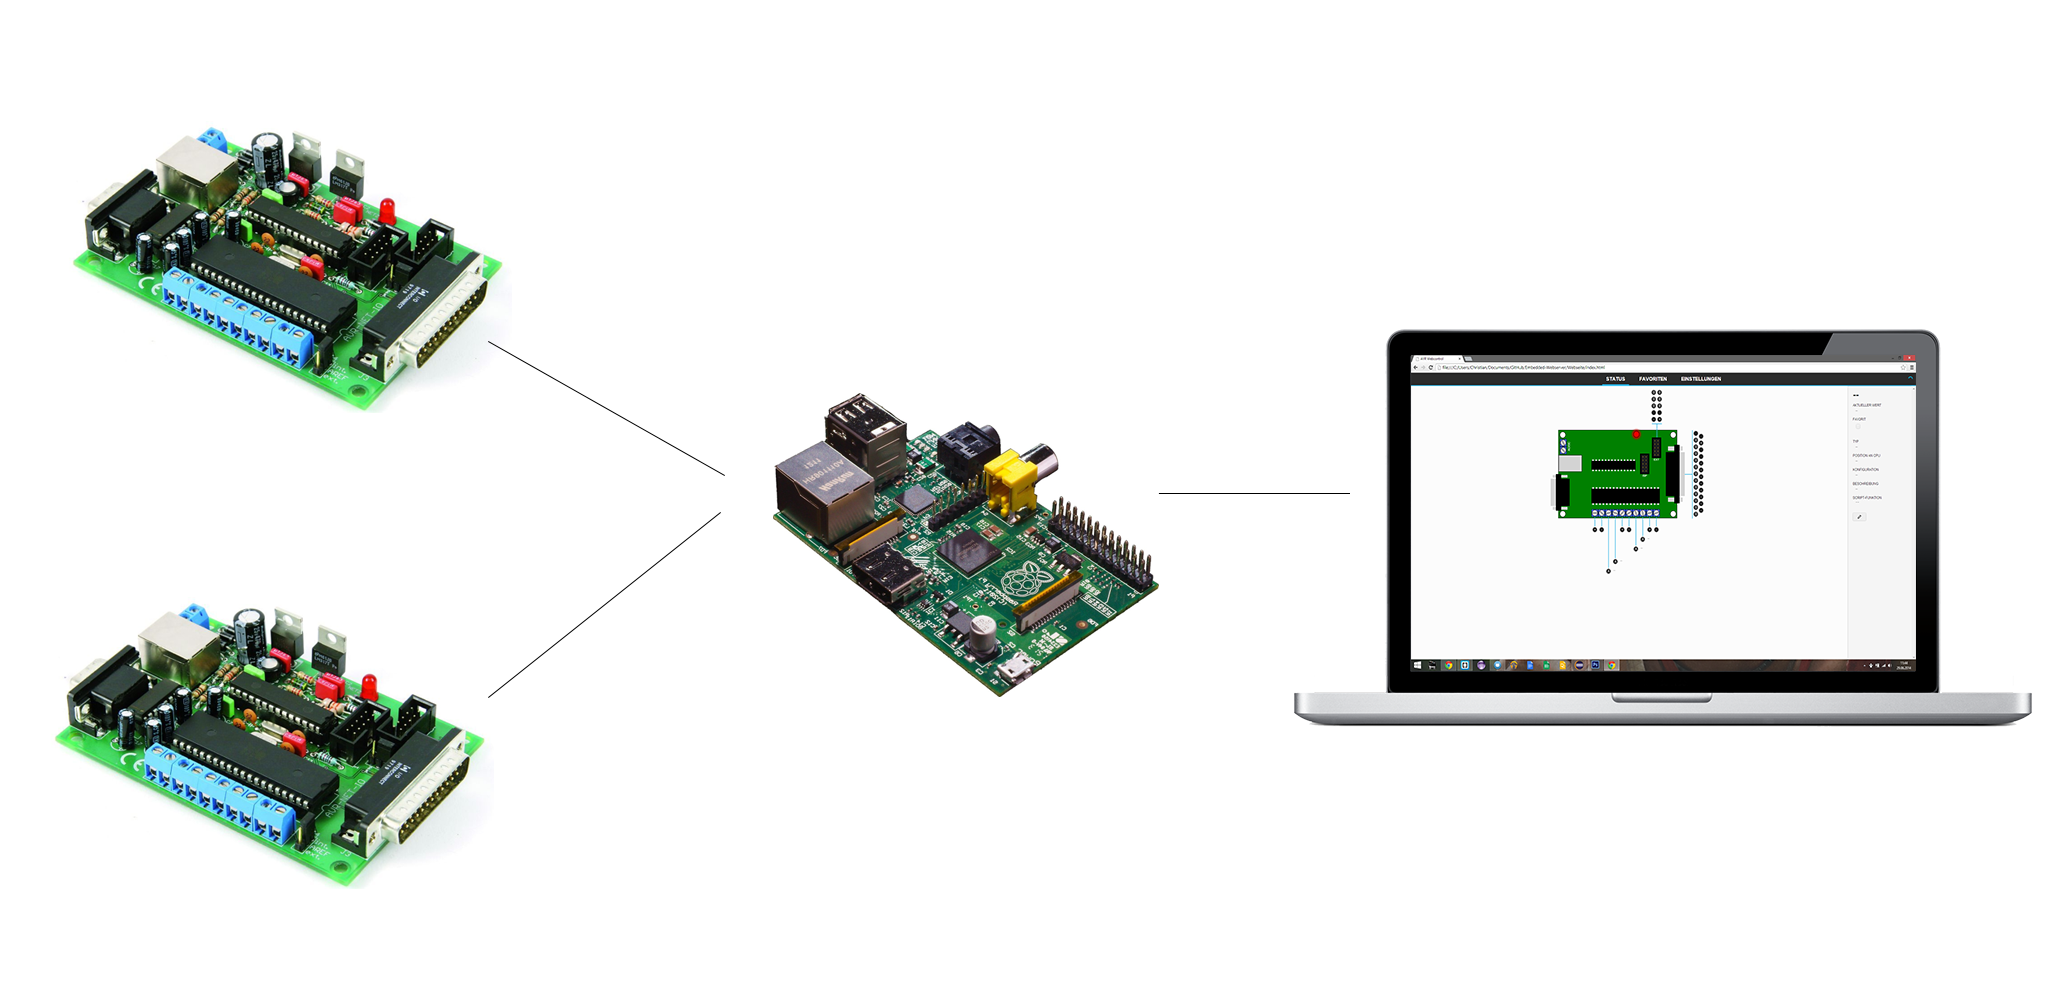
\includegraphics[width=13cm]{content/pictures/neues_system.png}
\caption{Der grobe Aufbau des neues Systems, links zwei Pollin Net-IO Boards,
in der Mitte ein Rasberry Pi und links ein Client}
\label{struktur}
\end{figure}
Die Clients fragen alle Daten, welche in einer kleinen Datenbank
zwischengespeichert werden, von dem zentralen Rasberry Pi ab. So ergeben
sich zwei Teilsysteme: \\
\\
Das erste besteht aus dem Rasberry Pi und den Pollin Net-IO Boards,
welche über die von Pollin bereit gestellte Schnittstelle kommunizieren.
Die Verwendung der bereits vorhandenen Schnittstelle macht es unnötig am
Microcontroller irgendwelche Änderungen vorzunehmen oder eine neue Firmware
flashen zu müssen, was die Usability enorm steigert, da das System auch von
Laien betrieben werden kann. Sobald neue Werte vorliegen sollten die Pollin
Net-IO Boards die Änderungen zum Rasberry Pi pushen, welcher die Werte in einer
kleinen Datenbank zwischenspeichert.Zur Verwendung des bestehenden Protokolls 
muss dieses mit Wireshark analysiert und reverse engineered werden. Hierfür 
kann die Netzwerkkommunikation des Pollin Net-IO Boards mit der mitgeliferten 
PC-Software beobachtet werden.\\
\\
Das zweite System besteht aus dem Rasberry Pi und den Clients. Die Clients
fragen über HTTP beim Server die Webseiten-Dateien und Messwerte ab. Die
Messwerte sollten nicht wie bei der aktuellen Lösung gepollt sondern nur bei
Bedarf mit Hilfe der im Kapitel "`Technischer Hintergrund"' erläuterten HTML5
Server-Sent Events Technik zum Client gepusht werden. Dies reduziert den
unnötigen Netzwerkverkehr. Ein Client kann immer nur ein Pollin Net-IO Board
darstellen, deshalb muss dem Nutzer auf der Webseite die Möglichkeit gegeben
werden, das darzustellende Board auszuwählen. Außerdem muss auf der Webseite die
zu verwendenden Boards (also welche der Rasberry Pi anspricht und den Clients
anbietet) konfiguriert werden können. Ansonsten ist die Webseite ohne große
Änderungen übernehmbar.

%-----------------------------------------------------------------------------------------
\section{Änderungen an der Webseite/Server-Schnittstelle}
\label{aenderung_schnitstelle}
Die Kommunikation zwischen Server und Webseite muss für die neuen Anforderungen
entsprechend erweitert werden. \\
\\
In einem ersten Schritt sollten alle REST-URLs um einen Parameter erweitert
werden, der das Pollin Net-IO Board identifiziert, von dem die Informationen
angefordert werden. Dies ist nötig, da das System über mehrere Boards
verfügen könnte. Der Parameter kann als HTTP-GET Parameter übergeben werden. Als
ID eignet sich z.B. die IP-Adresse des betreffenden Boards oder eine künstliche 
ID in Form einer fortlaufend höheren Zahl. Die aufzurufende URL wäre folglich
z.B. \textrm{/rest/values?id=192.168.2.6}.\\
\\
Danach sollte das aktuell über die POST-Parameter stattfindende
Setzen von Pins ebenfalls über die REST-Schnittstelle gelöst werden. Hierfür
müssen zwei neue URLs eingeführt werden, eine zum Setzen der Pinwerte und eine
zum Setzen des DDRs. Natürlich müssen auch die neuen URLs über den
Parameter zum identifizieren des betroffnen Boards verfügen.\\
\\
Zum Schluss muss noch eine URL bereitgestellt werden um eine Liste aller
verfügbaren Boards abfragen zu können. Zusätzlich muss noch eine URL zum
Hinzufügen eines neuen Boards und eine zum Entfernen eines vorhandenen Boards
angelegt werden.\\
\\
Sobald an der Webseite die Schnitstelle manipuliert wird, ist die Kommunikation
mit dem von uns entwickelten Server nicht mehr möglich. Das System kann nicht
mit HTTP-GET Parametern umgehen. Aus diesem Grund sollte zu Beginn der
Entwicklung ein Testserver aufgesetzt werden. Dieser kann aus einem lokalen
XAMPP-Server bestehen, welcher statt dynamisch Dateien für die
REST-Schnittstelle zu erzeugen über statische Dateien verfügt, welche mit
Testwerten gefüllt sind. So würde z.B. unter \textrm{/rest/pininfo} eine reale
Datei liegen, in der anstatt der Platzhalter feste Werte eingetragen sind. Dies
ermöglicht die Entwicklung der Webseite bzw. dem Ansprechen des Servers ohne
einen funktionsfähigen Rasberry Pi.

%-----------------------------------------------------------------------------------------
\section{Änderungen an der Webseite}
\subsection{Einstellungen}
Die meisten Änderungen der Webseite finden in den JavaScript Dateien statt. Alle
Einstellungen werden mit Hilfe von \textrm{db.js} gespeichert. Aktuell werden
die Einstellungen lokal gespeichert. Dies kann entweder beibehalten werden oder
die Einstellungen können zentral auf dem Rasberry gespeichert werden, was es
ermöglichen würde Favoriten etc. zwischen mehreren Clients zu synchronisieren.
Hierfür müsste nur der Speicherort geändert werden, an dem \textrm{db.js} die
Daten ablegt. Anstatt diese lokal zu speichern müssten sie zum Server geschickt
werden, welcher sie wiederrum an alle anderen Clients weiterleitet.

\subsection{Implementierung der neuen Schnittstelle}
Die neue Schnittstelle zwischen Server und Webseite muss natürlich implementiert
werden. Alle hierfür nötigen Änderungen finden in der \textrm{rest.js} statt.
Neben der Implementierung der Server-Sent Events um neue Messwerte zu
empfangen müssen auch neue Getter und Setter angelegt werden, um z.B. alle
vorhandenen Boards abfragen zu können.\\
\\
Aktuell wird die Funktion \textrm{refreshValues()} dazu verwendet, die Daten
zyklisch nachzuladen. Gestartet wird dieser Vorgang von 
\textrm{startNewRefreshTask()}. Diese Funktionen können in Folge der Umstellung
auf Server-Sent Events komplett gelöscht werden. Wichtig ist hierbei, dass die
Fuktion \textrm{setOnValuesChanged()} und das Attribut
\textrm{onValuesChanged} beibehalten wird. Indem \textrm{onValuesChanged()}
aufgerufen wird, wird \textrm{ui.js} darüber informiert, dass sich die Messwerte
geändert haben, was zur Aktualisierung der Oberfläche führt.

\subsection{Scriptfunktionen}
Aktuell gibt es zwei verschiedene Typen von Skriptfunktionen. Für jeden Pin
lässt sich eine Skriptfunktion zum Erstellen des dargestellten Messwertes
hinterlegen. Diese Skriptfunktionen müssen nicht geändert werden.\\
\\
Zusätzlich gibt es eine Skrtipfunktion die in den Einstellungen festgelegt
werden kann. Sie muss für jedes Board separat verfügbar und anpassbar sein.
Aktuell wird sie auf dem Clientsystem als JavaScript ausgeführt, dass hat zu
Folge das die Skriptfunktion nur so lange funktioniert, wie das Clientsystem
aktiv ist, also die Webseite also angezeigt wird. Diese Skriptfunktion sollte auf dem
Rasberry Pi gespeichert und ausgeführt werden.

\subsection{Auswahl des darzustellenden Boards}
\label{auswahl_board}
Da die Webseite immer nur ein Pollin Net-IO Board darstellen kann, muss dem
Nutzer eine Möglichkeit gegeben werden, eines aus allen verfügbaren auszuwählen.
Hierfür bietet es sich an im \textrm{div} Element mit der ID \textrm{header}
ein \textrm{select} anzubieten (z.B. auf der linken Seite, siehe
Abbildung \ref{select_board}), mit dem das darzustellende Board ausgewählt
werden kann.
Für die Positionierung des Elementes kann das \textrm{div} Element mit der ID
\textrm{loading\_loop} als Vorlage genutzt werden.

\begin{figure}[H]
\centering
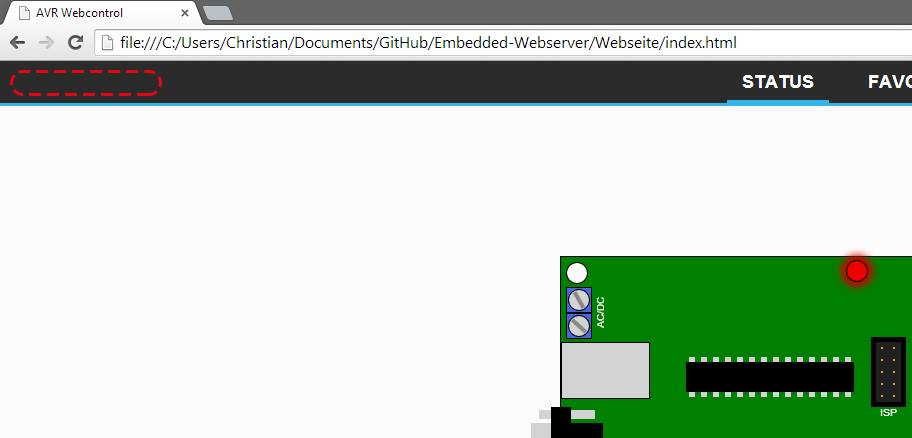
\includegraphics[width=13cm]{content/pictures/select_board.png}
\caption{Vorgeschalgene Position für ein select-Element um die darzustellende
Platine zu wählen}
\label{select_board}
\end{figure}

Beim Einfügen des \textrm{select} Elements in der Header ist zu beachten, dass die
Höhe des Headers nicht verändert werden sollte. Sollte dies dennoch nötig sein,
müssen die Kommentare im CSS-Code beachtet werden, um alle anderen nötigen
Änderungen durchzuführen.

\subsection{Verwaltung der Boards im System}
\label{verwaltung_system}
Im Einstellungs-Tab der Webseite muss eine Möglichkeit ergänzt werden, um die
neue Pollin Net-IO Boards zum System hinzuzufügen und vorhandene zu editieren
oder zu löschen. Für jedes Board sollte eine Sktipfunktion und ein Name
hinterlegbar sein. Der Name ermöglicht es dem Benutzer die Boards leichter
voneinander zu unterscheiden.

%-----------------------------------------------------------------------------------------
\section{Der neue Server}
Beim Server, welcher auf dem Rasberry Pi betrieben werden sollte, gibt es zwei
grundsätzliche Lösungsmöglichkeiten. Zum einen lässt sich der Server als
C/C++/Java-Programm realisieren, das einen Webserver zur Verfügung stellt oder
man realisiert den Server als PHP-Programm auf einem XAMPP-Server.\\
% Satz fängt mit "`zum einen"' an aber es kommt nie ein "`zum anderen"' ?? ..
\\
Bei beiden Alternativen muss der Server mit den einzelnen Pollin Net-IO Boards
kommunizieren, welche Daten über die REST-Schnittstelle bzw. die Server-Sent Events
bereitstellen sowie die Webseite hosten.

%-----------------------------------------------------------------------------------------
\section{Herangehensweise an das Projekt}
\subsection{Einpflegen des Rasberry Pi}
Im ersten Schritt sollte der Rasberry Pi in das bestehende System eingepflegt
werden. Hierfür sollte die Kommunikation zwischen Server und Webseite vorerst so
belassen werden wie sie aktuell ist, inklusive Polling. Der Server muss die
Daten von dem Pollin Net-IO Board empfangen (per Polling oder Pushing) und in
eine kleine Datenbank (oder ein Array etc.) hinterlegen. Bei jeder Abfrage der
Webseite werden die aktuellsten Daten weitergeleitet.\\
\\
Zu beachten ist, dass später die Skripte auf dem Server ausgeführt werden sollen.
Aus diesem Grund würde sich PHP als Programmiersprache anbieten, da PHP-Code,
der als Text vorliegt, direkt mit \textrm{eval()} ausgeführt werden kann.

\subsection{Betreiben mehrer Pollin Net-IO Boards}
Anschließend sollten mehrer Pollin Net-IO Boards betrieben werden können.
Hierfür muss die Server/Webseiten-Schnitstelle entsprechend dem Kapitel
\ref{aenderung_schnitstelle} überarbeitet werden. Die direkte Implementierung
der HTML5 Server-Sent Events ist empfehlenswert. Außerdem muss die Oberfläche
der Webseite um eine Auswahlmöglichkeit für das zu verwendende Board sowie eine
Konfigurationsmöglichkeit für die einzelnen Boards im System erweitert werden
(siehe Kapitel \ref{auswahl_board} und \ref{verwaltung_system}).

\subsection{Verlagern der Skriptfunktionen auf den Server}
Im letzten Schritt sollten die Skriptfunktionen, die nach jedem Neuladen der
Werte ausgeführt wird (aktuell im Settings-Tab einstellbar), auf dem Server
gespeichert und ausgeführt werden. Die Skriptfunktionen müssen natürlich von der
Webseite aus für jedes Board einzeln anpassbar sein. 
Wenn die Serverstruktur auf Basis des
XAMPP-Servers gewählt wurde, bietet sich PHP als Skriptsprache an, da der Code
nach dem Empfang neuer Werte direkt mit \textrm{eval()} ausgeführt werden kann.
Wichitg ist hierbei, dass über einfache Getter und Setter Funktionen der Zugriff
auf alle aktuellen Messwerte möglich ist und die Skriptfunktion auch Pins von
Boards sowie deren DDR manipulieren kann.

\chapter{Fazit}

Die Welt der Mikrocontroller steckt voller Möglichkeiten ist aber auch mit
einigen Schwierigkeiten behaftet. Anders als beim arbeiten mit Computern bei
denen der Speicherplatz für einfache Programme schier unbegrenzt ist kommt es bei
den Mikrocontroller auf jedes Byte an. So bestand in unserem Projekt nicht nur
die Schwierigkeit darin den Server mit weiteren Funktionen auszustatten sondern
auch bei der Programmierung möglichst auf Effizienz zu achten und den
bestehenden Webserver von nicht benötigten Funktionen zu befreien. Als eine
weitere Herausforderung bei Mikrocontrollern kommt noch die ganze elektronische
Seite hinzu. Als Informatiker haben wir durch das Studium kaum Berührung mit
diesem Thema gehabt und mussten uns vielerorts in die Themaktik einarbeiten.
Doch hat sich das Projekt als handhabbarer erwiesen als anfangs gedacht. Die
Hauptaufgaben bestanden hier im beschaffen von Bauteilen, dem
erstellen von Platinen zum Testen der Funktionen oder dem Programmieren und
Debuggen des Mikrocontrollers.



% Schalgwortverzeichnis (Index)
%\printindex

% Literaturverzeichnis
\singlespacing
\bibliographystyle{alphadin}
\bibliography{bibtex}

% Eidesstattliche Erklärung
%\include{content/affirmation}

\appendix
% Hier können Anhaenge angefuegt werden

\end{document}      